\pdfoutput=1

\documentclass[3p]{elsarticle}

\makeatletter
\def\ps@pprintTitle{%
 \let\@oddhead\@empty
 \let\@evenhead\@empty
 \def\@oddfoot{}%
 \let\@evenfoot\@oddfoot}
\makeatother

\journal{Journal of Process Control}

% *** GRAPHICS RELATED PACKAGES ***
\usepackage{graphicx}
\usepackage{pgfplots}
\usepackage{float}
\usepackage{caption}
\usepackage{subcaption}

% *** MATH PACKAGES ***
\usepackage{amsmath}
\usepackage{amssymb}
\usepackage{bm}
\usepackage{amsthm}

% *** SPECIALIZED LIST PACKAGES ***
\usepackage{algorithm}
\usepackage{algpseudocode}

% *** ALIGNMENT PACKAGES ***
\usepackage{array}

% *** PDF, URL AND HYPERLINK PACKAGES ***
\usepackage{url}

% *** TABLES PACKAGES ***
\usepackage{booktabs}
\newcommand{\ra}[1]{\renewcommand{\arraystretch}{#1}}

% *** USER DEFINITION ***
\newtheorem{Assumption}{\bf Assumption}

\newtheoremstyle{problemstyle} % <name>
        {3pt}                  % <space above>
        {3pt}                  % <space below>
        {\normalfont}          % <body font>
        {}                     % <indent amount}
        {\bfseries}            % <theorem head font>
        {\normalfont:}         % <punctuation after theorem head>
        {.5em}                 % <space after theorem head>
        {}                     % <theorem head spec (can be left empty, meaning `normal')>
\theoremstyle{problemstyle}

\newtheorem{Theorem}{Theorem}
\newtheorem{Problem}{Problem}
\newtheorem{Remark}{\bf Remark}

\begin{document}

\begin{frontmatter}

\title{Anomaly Detection in Wireless Sensor Networks Using Support Vector Data Description with Mahalanobis Kernels and Control Limit Adjustment}

\author[danang]{Van Vuong~Trinh\corref{cor1}}
\cortext[cor1]{Corresponding author}
\ead{vanvuong.trinh@gmail.com}

\author[danang]{Kim Phuc~Tran}

\author[hanoi]{Anh Tuan~Mai}

\address[danang]{Division of Artificial Intelligence, Faculty of Information Technology,\\ Dong A University, Danang, Vietnam} 
\address[hanoi]{International Training Institute for Materials Science (ITIMS),\\Hanoi University of Science and Technology, Hanoi, Vietnam} 

\begin{keyword}
Wireless sensor networks, Anomaly detection, Outlier detection, Support vector data description.
\end{keyword}

\begin{abstract}
\end{abstract}

\end{frontmatter}

\section{Introduction}

Wireless sensor networks (WSNs) \cite{Xie2011}

\cite{feng2017new}

\cite{Rajasegarar2014}

\subsection*{Notation and Definition}

$x \cdot y$ is inner product.

\section{Description of Anomaly Detection Approach}

In this section, we recall the so-called support vector data description (SVDD) originally derived in \cite{Tax2004}, which is an alternative of one-class support vector machines (OCSVM) \cite{scholkopf2001estimating} and is analogous to the known support vector machines (SVM) \cite{Vapnik1998}. Practical perspectives regarding modified discriminative function with control limit adjustment and hyperparameter selection based on Bayesian optimization are also discussed. Finally, an anomaly detection algorithm is summarized for clarity.

\subsection{Theory of SVDD}

Given $N$ samples $x_k \in \mathcal{X}$, $k=1,\dots,N$, SVDD method aims to estimate a sphere with minimum volume that contains all (or most of) these data. Let $a$ and $R$ being reserved for the center and the radius of the sphere, we define the objective function to minimize the volume of the sphere and the number of outliers as:
\begin{align}
R^2 + C \sum_{k=1}^N \xi_k
\end{align}
where $C > 0$ is a regularization parameter with constraints that almost data points are within the sphere:
\begin{align}
\left|\left| x_k - a \right|\right|^2 \le R^2 + \xi_k \text{, } \xi_k \ge 0 \text{, for } k=1,\dots,N
\end{align}

To adapt with nonspherical distribution, a conventional approach is to map given data into a higher dimensional feature space, namely $\mathcal{F}$, then learning a sphere in such a new space. This results into the so-called \emph{primal optimisation} as follows:
\begin{subequations}\label{eq:svm_primal}
\begin{align}
\underset{
	\begin{array}{c}
		 R, a, \xi
	\end{array}}{\text{Minimize }} &R^2 + C \sum_{k=1}^N \xi_k \\
\text{Subject to } &\left|\left| \phi \left( x_k \right) - a \right|\right|^2 \le R^2 + \xi_k \text{, } \xi_k \ge 0 \text{, for } k=1,\dots,N
\end{align}
\end{subequations}
where $\phi \left( \cdot \right): \mathcal{X} \to \mathcal{F}$ is the aforementioned feature mapping. The Lagrangian is hereafter written as:
\begin{align}
\mathcal{L} &= R^2 + C \sum_{k=1}^N \xi_k - \sum_{k=1}^N \alpha_k \bigg[ R^2 + \xi_k - \bigg( \phi \left( x_k \right) \cdot \phi \left( x_k \right) - 2 a \cdot \phi \left( x_k \right) + \phi \left( a \right) \cdot \phi \left( a \right) \bigg) \bigg] - \sum_{k=1}^N \gamma_k \xi_k \label{eq:svm_lagrange_init}
\end{align}
with the Lagrange multipliers $\alpha_k, \gamma_k \ge 0$. $\mathcal{L}$ should be minimized w.r.t. $R, a$ and maximized w.r.t. $\alpha_k, \gamma_k$.

Setting partial derivatives gives:
\begin{align}
\dfrac{\partial \mathcal{L}}{\partial R} = 0 &: \quad \sum_{k=1}^N \alpha_k = 1 \label{eq:svm_lagrange_dLdR} \\
\dfrac{\partial \mathcal{L}}{\partial a} = 0 &: \quad a = \sum_{k=1}^N \alpha_k \phi \left( x_k \right) \label{eq:svm_lagrange_dLda} \\
\dfrac{\partial \mathcal{L}}{\partial \xi_k} = 0 &: \quad \alpha_k + \gamma_k = C \label{eq:svm_lagrange_dLdxi}
\end{align}
Obviously, Lagrange multipliers $\gamma_k$ can be eliminated by imposing bound constraints on $\alpha_k$ as:
\begin{align}
0\le \alpha_k \le C
\end{align}
Then, substituting \eqref{eq:svm_lagrange_dLdR}-\eqref{eq:svm_lagrange_dLdxi} into \eqref{eq:svm_lagrange_init} leads to the following \emph{dual optimisation}:
\begin{subequations}\label{eq:svm_dual}
\begin{align}
\underset{
	\begin{array}{c}
		 \alpha
	\end{array}}{\text{Maximize }} &\sum_{k=1}^N \alpha_k \left( \phi \left( x_k \right) \cdot \phi \left( x_k \right) \right) - \sum_{k=1}^N \sum_{l=1}^N \alpha_k \alpha_l \left( \phi \left( x_k \right) \cdot \phi \left( x_l \right) \right) \\
\text{Subject to } &\sum_{k=1}^N \alpha_k = 1 \text{, } 0 \le \alpha_k \le C \text{, for } k=1,\dots,N
\end{align}
\end{subequations}
This standard quadratic program (QP) and can be solved more efficiently than the primal problem. Evidently, \eqref{eq:svm_dual} is feasible iff $C \ge \dfrac{1}{N}$ \cite{chang2013revisit}. Assume that such a feasibility condition holds, the following interpretation is trivial once \eqref{eq:svm_dual} is solved.
\begin{subequations}
\begin{align}
&\left|\left| \phi \left( x_k \right) - a \right|\right|^2 < R^2 \to \alpha_k = 0 \\
&\left|\left| \phi \left( x_k \right) - a \right|\right|^2 = R^2 \to 0 < \alpha_k < C \label{eq:sv_alpha}\\
&\left|\left| \phi \left( x_k \right) - a \right|\right|^2 > R^2 \to \alpha_k = C
\end{align}
\end{subequations}
Only data samples $x_k$ with $0 < \alpha_k < C$ are required in the distribution's description and these objects will therefore be refrered to as \emph{support vectors}. This will be discussed later after we generalize the linear SVDD into nonlinear version using kernel functions in the next sub-section. 

\subsection{Generalization with kernels}

Instead of using inner product, an alternative kernel product can also be adopted:
\begin{align}
\kappa \left( x_k, x_l \right) = \phi \left( x_k \right) \cdot \phi \left( x_l \right)
\end{align}
This is the known \emph{kernel trick} \cite{Scholkopf2001}, aims to avoid the need of explicitly declaring a feature mapping $\phi \left( \cdot \right)$. 

In this paper, we investigate the performance of SVDD using the Mahalanobis kernel (MHK):
\begin{align}
\kappa \left( x_k, x_l \right) = \exp \left( -\dfrac{ \left( x_k - x_l \right)'S^{-1}\left( x_k - x_l \right) }{2\sigma} \right)
\end{align}
where $S$ is the estimated covariance matrix computed with the available training data $x_k$, $k=1,\dots,N$ while parameter $\sigma$ is the kernel width. Then, we compare obtained result with the popular radial basis function kernel (RBFK, or Gaussian kernel):
\begin{align}
\kappa \left( x_k, x_l \right) = \exp \left( -\dfrac{ \left( x_k - x_l \right)'\left( x_k - x_l \right) }{2\sigma} \right)
\end{align}

Thus, the optimisation \eqref{eq:svm_dual} changes into:
\begin{subequations}\label{eq:svm_dual_kernel}
\begin{align}
\underset{
	\begin{array}{c}
		 \alpha
	\end{array}}{\text{Maximize }} &\sum_{k=1}^N \alpha_k \kappa \left( x_k, x_k \right)  - \sum_{k=1}^N \sum_{l=1}^N \alpha_k \alpha_l \kappa \left( x_k, x_l \right)  \\
\text{Subject to } &\sum_{k=1}^N \alpha_k = 1 \text{, } 0 \le \alpha_k \le C \text{, for } k=1,\dots,N
\end{align}
\end{subequations}
By solving this problem, one obtains the support vectors $x_i$, $i=1,\dots,m$ where $m$ is the number of support vectors. Then, sphere's radius is indeed the distance from any support vector, for instance $x_i$, to the sphere's center:
\begin{align}
R = \sqrt{\kappa \left( x_i, x_i \right) - 2 \sum_{i=1}^m \alpha_i \kappa \left( x_i, x_i \right) + \sum_{i=1}^m \sum_{j=1}^m \alpha_i \alpha_j \kappa \left( x_i, x_j \right)}
\end{align}

\subsection{Discrimination with control limit adjustment}

This sub-section aims to establish the discriminative function for detecting anomalies with preliminary discussion on robustness. Roughly speaking, the kernel distance, namely $d \left( z, a \right)$, between a test point $z$ and the center $a$ of sphere will be computed:
\begin{align}
d \left( z, a \right) = \sqrt{\kappa \left( z, z \right) - 2 \sum_{i=1}^m \alpha_i \kappa \left( z, x_i \right) + \sum_{k=i}^m \sum_{j=1}^m \alpha_i \alpha_j \kappa \left( x_i, x_j \right)}
\end{align}
Then, it is compared with an appropriate threshold. Such a threshold is then referred to as \emph{control limit} whose value is highly affects the probability of false negative rate (or false alarm).

A trivial choice of the control limit is sphere's radius $R$. This means that the data lies within the sphere will be categorized as anomalous. However, as suggested in \cite[Section~7.1]{shawe2004kernel}, it might be better to introduce a slack variable $\delta$ chosen \emph{a priori} into the discriminative function. This is due to the fact that there is no guarantee that the data point outside the sphere is anomalous.

Thus, we hereafter use the following function for inclusion, where $\mathcal{H}$ stands for the Heaviside function $\mathcal{H}(x) = 1$, if $x \ge 0$ and $0$ otherwise.
\begin{align}
f \left( z \right) &= \mathcal{H} \left( d - R^2 - \delta \right) \nonumber \\
&= \mathcal{H} \left( \kappa \left( z, z \right) - 2 \sum_{i=1}^m \alpha_i \kappa \left( z, x_i \right) - D \right) \label{eq:decision_fcn}
\end{align}
The constant $D$ can be pre-computed offline as:
\begin{align}
D = \kappa \left( x_i, x_i \right) - 2 \sum_{i=1}^m \alpha_i \kappa \left( x_i, x_i \right) + \delta
\end{align}

A probabilistic analysis on the affect of $\delta$ upon probability of the false alarm is available and is summarized as follows.
\begin{Theorem}{(\cite[Theorem~7.9]{shawe2004kernel})}
Fixed the slack variable $\delta > 0$ and the expected anomalies percentage $\lambda > 0$. The function $f$ defined in \eqref{eq:decision_fcn} returns $1$ on test points $z$ drawn according to the considered distribution with probability at most:
\begin{align}
\mathcal{P} \left( \delta, \lambda \right) = \dfrac{1}{\delta N} \sum_{k=1}^N \xi_k + \dfrac{6R^2}{\delta \sqrt{N}} + 3 \sqrt{\dfrac{ln \left( 2 {}/ \lambda \right)}{2N}}
\end{align}
\end{Theorem}
This theorem formalizes the intuition that small control limit implies high sensitivity to novelties. In this paper, we will study the variation of the upper bound $\mathcal{P} \left( \delta, \lambda \right)$ with different values of $\delta$ while fixing $\lambda=0.05$ is the usual choice in practice, i.e. $5 \%$ of anomalies. 

\subsection{Hyperparameter optimization}

Similar to other kernel methods, the hyperparameters's selection is critical and worthmentioning. Most of research use heuristic grid search while Bayesian optimization has been recently investigated. Following the latter approach, where a black-box nonlinear optimization problem is considered as follows:
\begin{subequations}\label{eq:param_opt}
\begin{align}
\underset{
	\begin{array}{c}
		 C, \sigma
	\end{array}}{\text{Maximize }} &J \left( C, \sigma \right) \\
\text{Subject to } & \dfrac{1}{N} \le C \le 1 \text{, } \underline{\sigma} \le \sigma \le \overline{\sigma}
\end{align}
\end{subequations}
whereas $\underline{\sigma}$ and $\overline{\sigma}$ are some positive bounds of $\sigma$. For simplicity, in this paper, we deploy the geometric mean accuracy (g-mean) for performance measure, i.e.
\begin{align}\label{eq:gmean}
J \left( C, \sigma \right) := g = \sqrt{Acc_+ \times Acc_-}
\end{align}
where $Acc_+$ and $Acc_-$ are \emph{true positive rate} and \emph{true negative rate}, respectively.

\subsection{Proposed algorithm for anomaly detection}

\begin{algorithm}[H]
\algnewcommand{\LeftComment}[1]{\Statex \(\triangleright\) #1}
\renewcommand\algorithmicdo{until convergence}
\renewcommand\algorithmicfor{For}
\algtext*{EndFor}
\algrenewcommand\alglinenumber[1]{\normalfont #1}
\caption{(Anomaly detection algorithm) Given $\lambda > 0$ and $\delta > 0$, this algorithm optimizes SVDD's hyperparameters $(C,\sigma)$. Let $s$ being reserved for the iteration counter of an optimization solver $\mathcal{S}$. It requires training samples $\{ x_k^{train} \}_{k=1}^{N_{train}}$ and testing samples $\{ x_k^{test}, y_k^{test} \}_{k=1}^{N_{test}}$.}
\begin{algorithmic}[1]
\LeftComment{Training phase:} 
\State Initialize hyperparameters as $(C^{(0)},\sigma^{(0)})$.
\For{$s=1,2,\dots$}
\State Given $(C^{(s)},\sigma^{(s)})$ by the solver $\mathcal{S}$, solve \eqref{eq:svm_dual_kernel} with data set $\{ x_k^{train} \}_{k=1}^{N_{train}}$.
\State Validate the SVDD with data set $\{ x_k^{test}, y_k^{test} \}_{k=1}^{N_{test}}$, then compute $g$ according to \eqref{eq:gmean}.
\State Return $J \left( C^{(s)},\sigma^{(s)} \right) = g$, the solver $\mathcal{S}$ updates  the next iterate $(C^{(s+1)},\sigma^{(s+1)})$.
\EndFor
\State Return $(C^\star,\sigma^\star)$.
\LeftComment{Decision phase:} 
\State For an unknown sample $z$, classify it according to \eqref{eq:decision_fcn}.
\end{algorithmic}
\end{algorithm}

\section{Simulation Results}

This section investigates the efficiency of anomaly detection algorithm using Mahalanobis kernel and control limit adjustment over a real data set. Dual optimisation of SVDD was solved using the IBM ILOG CPLEX solver while hyperparameter optimization was conducted using the DIRECT algorithm \cite{gablonsky2001locally} implemented in the NLopt nonlinear optimization package \cite{nlopt}. All computation was performed on a platform with 2.6 GHz Intel(R) Core(TM) i7 and 16GB of RAM.

\subsection{Data description}

We consider a data set gathered from a wireless sensor network deployment at the Intel Berkeley Research Laboratory (IBRL) \cite{Buonadonna2005}. A wireless sensor network consisting of $54$ \emph{Mica2Dot} sensor nodes was deployed in the IBRL for a $30$ day ($720$ hour) period between 28th Feb 2004 and 5th April 2004 [10]. The sensors collect five measurements: light in Lux, temperature in degrees celsius, humidity (temperature corrected relative humidity) ranging from $0\%$ to $100\%$, voltage in volts and network topology information in each $30$ second interval. Node $0$ is the gateway node. Other nodes transmit their data in multiple hops to the gateway node. The furthest node in the network is about $10$ hops away from the gateway node. During the $30$ day period, the $54$ nodes collected about $2.3$ million readings.

In this paper we consider the IBRL data set obtained from $5$ close nodes, $1, 2, 33, 35, 37$. Also, only two features, namely temperature and humidity, are taken into account. The data during the first $10$ days period on March 2004 will be used as the training set while validation is performed upon the whole available data.

\subsection{Results}

\begin{figure}[H]
\centering
%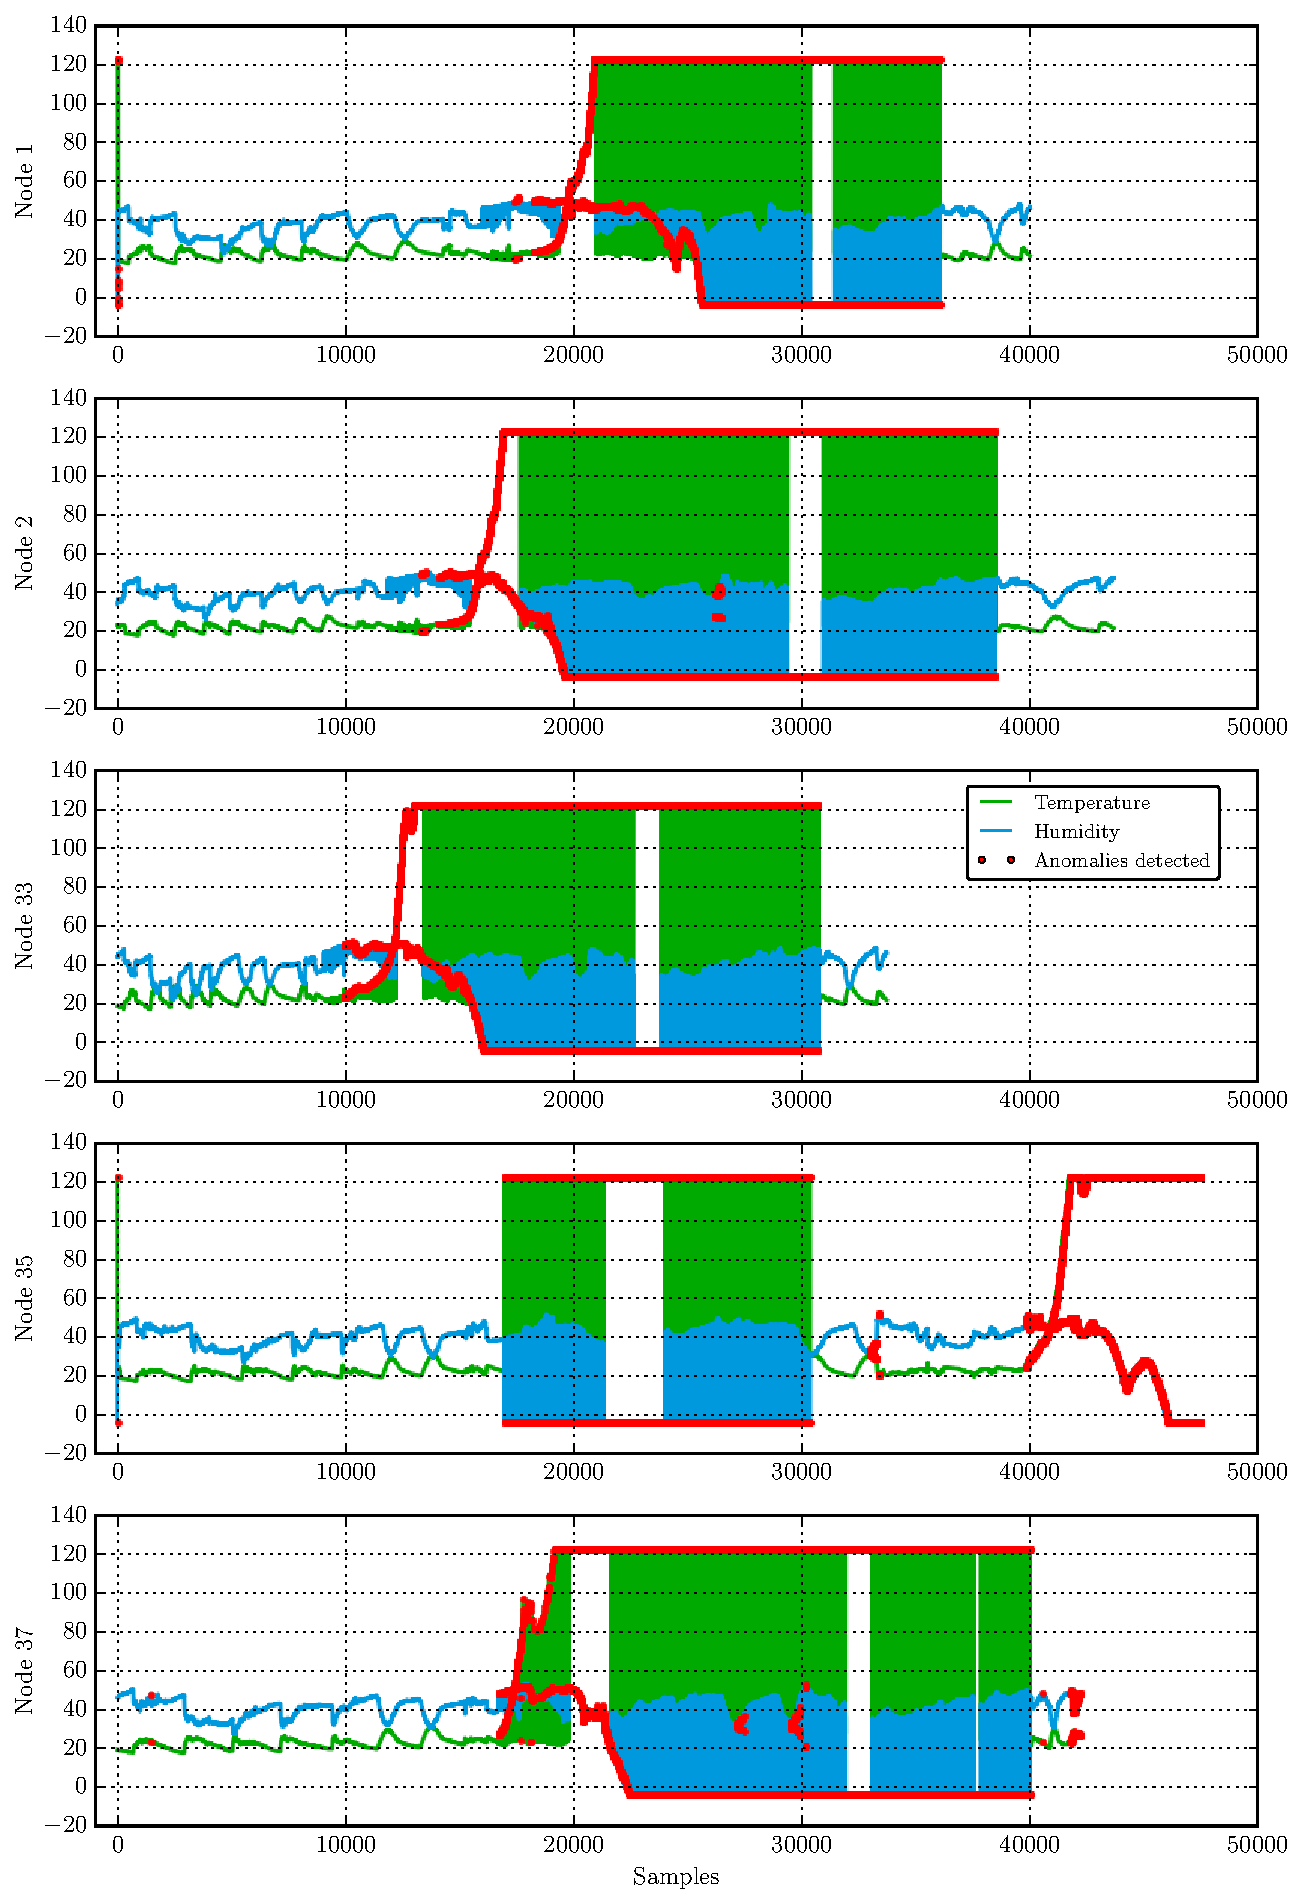
\includegraphics[scale=.6]{Figs/time_validation.pdf}
\caption{Time-domain validation using the anomaly detector with $\delta=0.02$.}
\end{figure}

x la data index
y la control limit distance

\subsection{Accuracy analysis}

\begin{figure}[H]
\centering
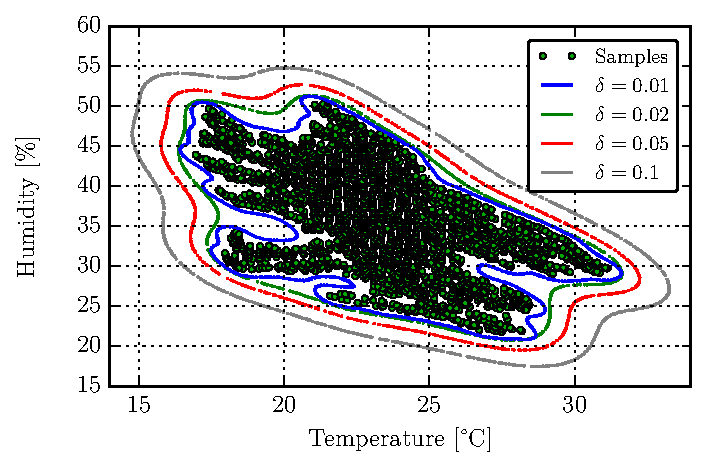
\includegraphics[scale=.6]{Figs/data_description.pdf}
\caption{Discrimination with different values of $\delta$.}
\end{figure}

\subsection{Robustness analysis}


\subsection{Comparison between MHK and RBFK}


\section{Conclusion and Future Work}



\bibliographystyle{IEEEtran}
\bibliography{wsnbib,svmbib,ocsvmbib,ibrlbib,miscbib}

\end{document}


